\subsection{BinAuth and Software IDs}
\label{sec:binauth-scheme}

We now present our binary authentication system, BinAuth.
We want a lightweight binary authentication scheme which can work
under many settings without too much reliance on other infrastructure.
Furthermore, it should help in the management of binaries, and incurs low overhead.
Management of binaries includes determining which binaries should be
authentic, dealing with issues arising from disclosed vulnerabilities,
and software patching.

\subsubsection{Software ID Scheme}

% \TODO{Cover the case if binary is not signed by developer.
% Remember we want to be lightweight so there are a few possibilities.
% The MAC can be computed at install/first use or it could be signed with
% a digital signature by the user/system administrator with a well known
% public key.}

We complement binary authentication with a software ID scheme meant
to simplify binary management issues.
The idea is that a {\em software ID} associates a
unique string to a particular binary of a software product.
The software ID should come either from the software developer
or alternatively be assigned by the system administrator.
The key to ensuring unique software\_ID, even among different
software developers, lies on the standardized format of the ID.
We can define software\_ID as follows:
\begin{center}
\small
Software\_ID ::= $\langle$ opcode\_tag $\mid\mid$ vendor\_ID $\mid\mid$ 
product\_ID $\mid\mid$ module\_ID $\mid\mid$ version\_ID$\rangle$.
\footnote{Module\_ID suffices to deal with software versioning.
Having a separate version\_ID, however, is useful to easily
track different versions (or patched versions) of the same program.}
\end{center}
\noindent 
Here, $\mid\mid$ denotes string concatenation.
Opcode\_tag distinguishes different naming convention, eg.
$Software\_ID$ and $Custom\_ID$ defined below.

Ideally, we want to be able to uniquely assigning vendor\_IDs to
producers of software which can make the software\_ID unique.
This problem in practice might not be as difficult as it sounds since
it is similar to domain name registration or the assignment
of Medium Access Control (MAC) addresses by network card manufacturers.
One can leverage on existing trust infrastructures to do this.
For example, the responsibility for unique and well known software\_IDs
can be assigned to a Certificate Authority (CA), which then 
define the vendor\_ID as $\langle$ CA\_ID $\mid\mid$ vendor\_name $\rangle$. 
Alternatively, one might be able to use the domain name of the 
software developer as a proxy for the vendor\_ID.

% as
% As we see an increasingly common trend of software developers having
% a certificate, it is thus possible that the assignment responsibility be
% collocated to Certificate Authority (CA). The CA can establish 
% trust management of this software issuer, possibly by including
% added information in the certificate.
% Thus, vendor\_ID ::= $\langle$ CA\_ID $\mid\mid$ vendor\_name $\rangle$
% is sufficient to guarantee unique vendor string information.
%Another example would be the domain name registration where the responsibility
%is also co-located in a organized hierarchical way.

A software\_ID gives a one to one mapping between the binary and its ID string.
This is useful for dealing with vulnerability management problems \cite{sufatrio2004amo}.
Suppose a new vulnerability is known for a particular version of a software.
This means that certain binaries, providing that they correspond to that
software version may be vulnerable. However, there is no simple and standard
way of automatically determining this version information.
Once we have software\_IDs associated with binaries then one can check
the software\_ID against vulnerability alerts. The advisory may
already contain the software\_ID. 
Automatic scanners can then be used
to tie-in this checking with the dissemination of vulnerability alerts
to automatically monitor/manage/patch the software in an operating system.
General management of patches in an operating system can also be done
in much the same way.

In the case where no software\_ID comes with a software product,
one can alternatively derive one.
It can be constructed, for instance, using the following (coarse-grained) string naming:
\begin{center}
\small
$Custom\_ID$ ::= $\langle$ opcode\_tag $\mid\mid$
$hash$(vendor\_URL + product\_name + file\_name + salt) $\rangle$.
\end{center}
The salt expands the name space to reduce the risk of a hash function collision.
% This strategy should provide us with a reasonably reliably mechanism 
% to assign a unique string provided that no collision due to the hash function occurs.

\begin{figure}[tb]
\begin{center}
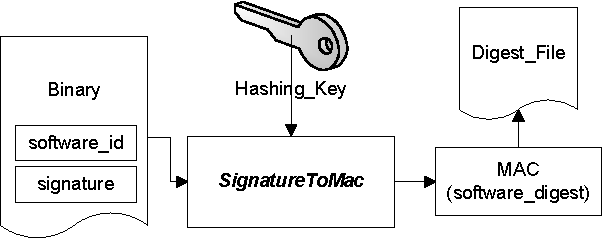
\includegraphics[width=0.6\textwidth]{binauth/hashing}
\caption{SignatureToMac: Deriving the MAC}
\label{fig:hashing}
\end{center}
\end{figure}

\subsubsection{BinAuth System Architecture}

% \TODO{Password issues:
% Password not stored on the machine.
% During the early part of boot, the password could be entered into
% the system or obtained through any secure means which is outside the control
% of the machine.
% What about user passwords?? Still going to have it or not??
% Its feasible but one still has to deal with the boot phase.}

% The key to our lightweight authentication is the derivation
% of a MAC from a binary's valid digital signature.

In the following discussion, we assume here that binaries already come 
tagged with a software\_ID. 
During the BinAuth set-up, preferably done immediately after 
the targeted binary installation, we generate the MAC values for each binary.
In the case where binaries are digitally signed by its developer,
then we verify the signature and then generate the MAC for each binary.
Thus, only one public-key operation needs to be done at install time.
We choose to use a keyed hash, the HMAC algorithm \cite{krawczyk1997rfc2104},
so there is a secret key for the administrator. This is mainly to increase
the security of the stored hashes.
To authenticate binary integrity for any future execution of the code,
only the generated HMAC needs to be checked.
% NO space
% \footnote{
% There are subtle trust issues 
% in the event of certificate expiration/revocation, 
% see Sec. ~\ref{sec:binauth-analysis}.}
In what follows, we mostly write MAC which already covers the choice of HMAC.

One way of storing the generated MAC is by embedding it into the binary.
However, doing so may interfere with file format of the signed binaries
and may also have other complications. 
We instead use an authentication repository file
which stores all the MAC values of authenticated binaries
with their pathnames.
During the boot-up process, the kernel creates its own in-memory data structures
for binary authentication from this file. 
We ensure that the repository file is protected from further modification
except under the control of the authentication system to 
add/remove binaries.\footnote{
Further security can be achieved by integrating binary authentication
with a TPM infrastructure. We do not do so in the prototype as that is
somewhat orthogonal.
}
We can also customize BinAuth on a per user basis rather
than system-wide which is a white-list of
binaries approved for execution.
% Having a MAC repository like this additionally allows us to
% perform the authentication per user basis rather than system-wide.
% Each user in the system thus can have his/her own list of approved binaries.
% This infrastructure thus can readily implement user's application control list
% as in \cite{EMU}.
In the case, when the initial binary does not have a digital signature, then
the administrator can still choose to approve the binary and generate a MAC
for it.

There are two main components of the system: the {\bf SignatureToMac} and {\bf Verifier}.
The SignatureToMac maintains the authentication repository, {\it Digest\_file}, 
consisting of $\langle$path, MAC$\rangle$ tuples.
The Verifier is a kernel driver which makes use of
{\it Digest\_file} and
decides whether an execution is to be allowed.

%\subsubsubsection{SignatureToMac}
\paragraph{SignatureToMac}

Once software is installed on the system,
Fig. \ref{fig:hashing} shows how SignatureToMac processes the binaries:
\begin{enumerate}
\item Checks the validity of the binary's digital signature.
If the signature is invalid, then report failure.
%This step is one where public-key and PKI operation are ever done for each binary.
\item It consults the user or system administrator whether 
the software is to be trusted or not (this is similar to the Vista UAC 
dialog but only happens once).
Other policies (possibly mandatory) can also be implemented.
\item It generates the MAC of the binary 
(including software\_ID string) using a secret key, {\it Hashing\_key}, 
to produce {\it software\_digest}.
The {\it Hashing\_key} is only accessible
% stored in a protected file which can only be accessed 
by the authentication system, e.g. obtained on bootup.
\item It adds an entry for the binary as a tuple $\langle${\it path name}, 
{\it software\_digest}$\rangle$ into the {\it Digest\_file} repository
and informs the Verifier.
The repository is protected against modification. Note that because the entries
are signed, the repository can be read for other uses, e.g.
version control and vulnerability management.
\end{enumerate}

% In order to ensure smoother authentication of all binaries on a system,
% there ideally should be a mechanism that allows system administrator to 
% list all newly added binaries after a software installation.
% Complying installer is thus appreciated to produce such list;
% or alternatively the administrator can deploy a tool 
% which monitors binaries addition during installation.

\begin{figure}[tb]
\begin{center}
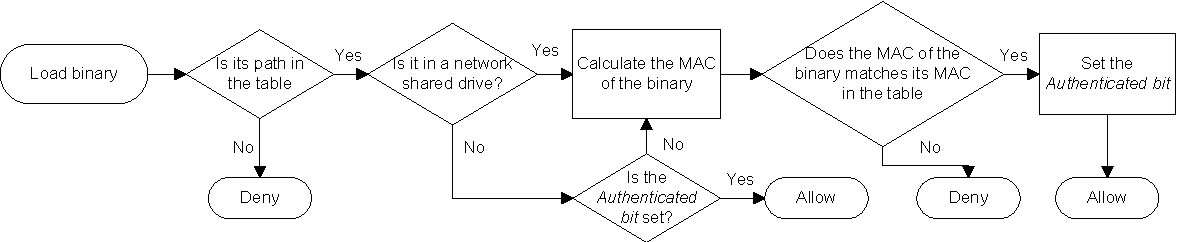
\includegraphics[width=1.0\textwidth]{binauth/verifier}
\caption{Verifier: The Verifier in-kernel authentication process}
\label{fig:verifier}
\end{center}
\end{figure}


%\subsubsubsection{Verifier}
\paragraph{Verifier}

% The Verifier initializes itself from {\it Digest\_file}.
The Verifier performs mandatory binary authentication ---
it denies the execution of any kind of Windows binary which
fails to match the MAC and pathname.
There are two general approaches for the checking.
One is {\em cached MAC} which avoids generating the MAC for
previously authenticated binaries.
The other is {\em uncached MAC} which always checks the MAC.
As we will see, they have various tradeoffs.
The cached MAC implementation needs to ensure that binaries are unmodified.
Hence, the Verifier monitors the usage of previously authenticated files 
on the cache, and removes them from the cache if it can be potentially modified.

The core data structure of the Verifier component can be viewed
as a table of tuples in the form
$\langle${\it Kernel\_path}, {\it FileID}, {\it MAC}, 
{\it Authenticated\_bit}$\rangle$
representing the allowed binaries.
It is indexed on {\it Kernel\_path} and {\it FileID} for fast lookup.
The fields are as follows:
\begin{itemize}
\item The {\bf {\it Kernel\_path}} is Windows kernel (internal) pathname 
representation of a file.
In Window's user space, a file can have multiple absolute pathnames, due to:
(i) 8.3 file naming format, e.g.
``{\tt C:\linebreak[0]$\backslash$\linebreak[0]Program Files\linebreak[0]$\backslash$\linebreak[0]}''
and
``{\tt C:\linebreak[0]$\backslash$\linebreak[0]progra$\sim$1\linebreak[0]$\backslash$\linebreak[0]}''
are the same;
(ii) symbolic links (reparse points is similar);
% to directories/files;
(iii) hard links;
(iv) volume mount points;
% \cite{ntfs-junction} 
or
(v) the {\tt SUBST} and {\tt APPEND} DOS commands.
% \cite{subst}.
The {\it Kernel\_path} is a unique representation for all
the possible pathnames.
% In the kernel, different pathnames referring to the same file 
% are resolved to a unique kernel name, which we use here.
When the system loads $\langle${\it path name}, {\it software\_digest}$\rangle$ 
from {\it Digest\_file} during the startup, {\it path name} is converted to 
{\it Kernel\_path} since all subsequent checks by Verifier in the kernel 
all use the latter.

\item The {\it FileID} is a pair of $\langle${\it device\_name}, {\it NTFS\_object\_ID}$\rangle$.
The {\it device\_name} is a Windows internal name to identify a 
disk or partition volume.
For instance, the device name {\tt HarddiskVolume1} usually refers to {\tt C:$\backslash$}.
The {\it NTFS\_object\_ID} is a 128-bit length number uniquely identifying
a file in the file system volume (this is not the same as Unix inode numbers)
% \cite{objid}.
The Verifier uses the {\it FileID} 
% \cite{hardlink}.
to identify the same file given more than one hard link.
This prevents an attacker from creating a hard link for modifying
a binary without invalidating the binary cache.
The {\it FileID} values will be queried from the system and 
filled into the table during system boot.

\item The {\it MAC} is same as a {\it software\_digest} entry in {\it Digest\_file}.
Our prototype implements the
HMAC-MD5 \cite{krawczyk1997rfc2104}, HMAC-SHA-1 
and HMAC-SHA-256 \cite{eastlake2006rfc4634} hash algorithms.\footnote{
Due to recent concerns which show weaknesses and attacks against MD5 \cite{wang2005break}, 
we also have stronger hash functions, namely SHA-1 and the stronger SHA-256.}
\item The {\it Authenticated\_bit} remembers whether the binary has
been previously authenticated.
It is initially set to false, and set to true after successful authentication.
\end{itemize}

\noindent
Fig. ~\ref{fig:verifier} shows the authentication process 
when a binary executes/loads:
\begin{enumerate}
\item It checks if the binary's {\it Kernel\_pathname} exists in the table.
If not, then deny the execution and optionally log the event.
A notification is accordingly sent to the user. 
% asking to first perform {\it SignatureToMac} step.
\item It the file is on a network shared drive, goto step 4.
The MAC is always
recomputed as we cannot keep track of modification to files on network shares.
\item If the {\it Authenticated\_bit} is set go to step 7.
\item It performs MAC algorithm operation on the binary.
\item If the resulting MAC doesn't match with the 
{\it MAC} stored in the table, execution is denied.
\item It sets the {\it Authenticated\_bit} of the binary.
\item It passes the control to the kernel to continue the execution.
\end{enumerate}

To control binary execution, we intercept the section creation action 
({\tt NtCreateSection()} system call) which is better than:
% As also discussed in \cite{bassov}, intercepting ({\tt NtCreateSection()}
% is a better option than two other alternatives:
\begin{itemize}
\item Intercepting file opening ({\tt NtCreateFile()} and {\tt NtOpenFile()}).
This would need to authenticate any file opened with with execute access mode.
As discussed in Sec.~\ref{sec:binauth-windows}, however, this introduces
unnecessary overheads and can cause some correct programs to fail if the files
do not pass authentication.
There are also technical difficulties to distinguish between
process creation and regular file IO operations, which is not always easy given
its microkernel nature.
%  \cite{bassov}.
\item Intercepting process creation ({\tt NtCreateProcess()}).
This method is not effective for our purpose.
%since it is possible to create a process without calling this system call,
%such as {\tt CreateProcess()}.
Firstly, we cannot use it to control {\tt DLL} loading.
Secondly, it is more difficult to get the pathname of the binary because
process creating is broken down into microkernel operations.
\end{itemize}
It turns out that since all code from any kind of binary
needs to have a memory section to execute,
it suffices to intercept {\tt NTCreateSection()}.

The cached MAC verifier needs to ensure that binaries which have
been already authenticated are not modified.
However, the uncached verifier will not need to perform file monitoring.
%For each entry of the table, we use the {\it Authenticated\_bit} 
%in order to keep track of whether the binary has been previously authenticated.
%Initially, all these bits are set to false.
%The bit is set to true when the binary is authenticated, and set back to
%false when the binary is modified.
A binary with pathname $P$ is considered modified, if the following occurs:
\begin{itemize}
\item $P$ is created: Hence, we monitor system call
{\tt NtCreateFile()} and {\tt NtOpenFile()}.
\item $P$ is opened with write access mode: the previous two
system calls are also intercepted for this purpose.
\footnote{An alternative way is to monitor the file (block) writing operation ({\tt NtWriteFile()}).
However, it is less efficient because file block writings take place more frequently
than file openings as one opened file for modification might be subject to 
multiple block writings. Furthermore, it cannot capture file-memory mapping.}
\item Another file is renamed to $P$: 
We monitor file renaming ({\tt NtSetInformationFile\linebreak[0](\linebreak[0]FileRenameInformation\linebreak[0])})
system call.
\item A drive containing $P$ is mounted:
We monitor drive mounting {\tt IRP\_MJ\_VOLUME\_MOUNT}.
\end{itemize}

\noindent
Note that we do not need to monitor file deletion since we only care about
executing correct files but not missing files.
The details of file modification monitoring are given in Fig. \ref{fileopen}.

Upon modification of $P$, we reset the {\it Authenticated\_bit} of binary $P$, 
and update the {\it FileID} in the table if it is changed.
Should FAT file system be used, pathname is used 
to identify the binary as {\it FileID} is not supported but
neither are hard and soft links.
% Additionally, hard links will not cause any security problems in FAT
% as they are not supported. 
Since {\it FileID} is optional and can be removed,
we monitor {\it FileID} removal ({\tt NtFsControlFile(FSCTL\_DELETE\_OBJECT\_ID)})
and deny the removal if the {\it FileID} is in the table.
Dut to the semantics of NTFS, our use of {\it FileID} can
coexist with other applications using it.

If additional hardware and infrastructure is available to support
secure booting, such as the Trusted Platform Module (TPM) initiative,
the system can benefit from increased security.
Offline attacks would have to first attack the TPM.
The Hashing\_key can also be stored securely by the TPM.

% In an infrastructure where additional hardware is available to ensure secure startup,
% such as recent initiative of Trusted Platform Module (TPM),
% then increased security level can be expected on the authentication system.
% For instance, the Hashing\_key can then be securely stored on the chip
% as opposed to the file system.
% Note that, due to the closed-source nature of Windows,
% it is hard to ensure completeness and soundness with regard to file modification monitoring.
% However, the outlined mechanisms should be sufficient
% to measure the effect of system overheads to provide cache mechanism in
% real-world OS like Windows.

\begin{figure}[tb]
\scriptsize
\begin{center}
\begin{verbatim}
procedure UponModification (FilePath)
   if (FS is NTFS)
      FileID := GetFileID(FilePath) # FileID can be NULL
      if (FilePath is in the table)
         Entry := LookupTableByPath(FilePath)
         if (FileID == NULL)
            # this can happen when the file is deleted and created again.
            # generate a new FileID and update the table
            Entry.FileID := CreateFileID(FilePath)
         else if ( FileID != Entry.FileID in the table)
            # this can happen when the drive is unmounted,
            # id changed off-line and re-mounted
            Entry.FileID := FileID
         end if
         Entry.Authenticated := false
      else if ((FileID != NULL) AND (FileID is in the table))
         Entry := LookupTableByID(FileID)
         Entry.Authenticated := false
      end if
   else if ((FS is FAT) AND (FilePath is in table))
      Entry := LookupTableByPath(FilePath)
      Entry.Authenticated := false
   end if
end procedure
\end{verbatim}
\end{center}
\caption{Pseudo code of file modification monitor}
\label{fileopen}
\end{figure}
\subsubsection{Security Analysis}
\label{sec:binauth-analysis}

The security of BinAuth relies on the strength
of the chosen hash functions (MD5, SHA-1, SHA-256) as well as
the HMAC algorithm.
Thus, we assume that any change in a binary can be detected through a changed MAC.

In our authentication on binary with digital signature, 
the subsequent invocations using MAC verification is sufficient 
to ensure the authenticity of the binary.
In other words, MAC authentications ``{\em preserve}'' the previously
established properties of BinAuth derived from digital signature.
A subtlety comes when the certificate expires or is revoked 
at some point in time after SignatureToMac.
We view that the question of whether one should keep trusting the binary for execution
depends on one's level of trust on certificate expiration/revocation.
If the certificate expiration or revocation means 
that the public key must no longer be used,
but the fact that {\em previously established} goodness binary properties still hold,
then we can keep trusting the binary for execution (as long as we still believe the issuer).

% \item {\it ``Provided that the Hashing\_key is good, any corruption of
% a binary's  software\_digest (MAC) in Digest\_file will result in a failed verification''}:\\
% %Informal Proof:\\
% As the hash on the binary is done with Hashing\_key,
% any corrupted software\_digest will thus result in a mismatch.
% This higher level of protection guarantee is the reason
% why we employ MAC algorithm (using Hashing\_key) instead of keyless hash operation.
% Although we can assume that digest\_file is stored securely,
% having a separate Hashing\_key provides increased protection.
% A highly secure system can then be achieved, for example, by having
% Hashing\_key stored in a more secure (tamper-resistant) storage.
% Given the key's short length, thus only very small memory requirement 
% on the storage is imposed in trade of higher security guarantee.
% \end{itemize}

% \subsubsection{Threat Analysis}
Here we discuss some possible attacks to the authentication system.
All the attacks except the last two target the caching system.
More precisely, the attacker attempts to modify an already authenticated
binary without causing the {\it Authenticated\_bit} to be set to false.

\begin{itemize}
\item {\bf Manipulating symbolic links:}
The attacker can use the path $S$ which is a symbolic link of an authenticated $P$
to indirectly modify $P$ and subsequently execute $P$.
However, the modified file will not be executed successfully, because
Windows kernel resolves symbolic links to real paths.
More precisely, the symbolic link $S$ is resolved to the real path $P$.
As a result, the {\it Authenticated\_bit} of $P$ will be set to false.
When $P$ is executed, its MAC will be recalculated and it will not pass
the authentication.

\item {\bf Manipulating hard links:}
The attacker can create a hard link $H$ on an already authenticated file $P$
and then modifies the file using path $H$.
This attack will not succeed because we use {\it FileID} to identify files.
$H$ has the same {\it FileID} as $P$,
thus the {\it Authenticated\_bit} will be set to false.
Note that this attack will not succeed in FAT file system either,
even though we cannot use {\it FileID}.
This is because hard link is not supported in FAT.

\item {\bf Manipulating FileID:}
Recall that {\it FileID} consists of {\it device\linebreak[0]\_\linebreak[0]name}
and {\it NTFS\linebreak[0]\_\linebreak[0]object\linebreak[0]\_\linebreak[0]ID}.
The latter is optional and thus can be removed.
The attacker can remove the {\it NTFS\_object\_ID}, and then performs the previous attack.
We handle this attack by denying {\it NTFS\_object\_ID} removal on authenticated files.
This is implemented by monitoring the file system control event {\tt FSCTL\_DELETE\_OBJECT\_ID}

\item {\bf Remote File Systems:}
Since we cannot keep track of modification on a network shared file system,
we do not cache the authentication.
More precisely, the MAC of the binary is always calculated upon loading.
Same applies to removable media such as floppy in which we can not
keep track of modification of files.

\item {\bf TOCTTOU:}
TOCTTOU stands for Time-Of-Check-To-Time-Of-Use.
It refers to a race condition bug of an access control system
where the resource is changed during the time
of checking the resource to the time of using the resource.
In the BinAuth context, the binary may be modified
after the time it is authenticated and before the time it is executed.
However, we observed that all binaries are exclusive-write-locked
when it is opened.
That means binaries cannot be modified from the time it is opened
to the time it is closed.
Also note that the file is authenticated after it is opened and before
it is executed.
As a result, binaries cannot be modified during TOCTTOU.

When the binary is in a network shared volume, i.e. SMB share,
and the write-lock is not properly implemented in the SMB server,
an attacker is able to modify the binary after authentication.
However, we have observed that both Windows and Samba
implement write-lock properly.
Thus the attack is only possible when the SMB server is compromised.
One way to prevent this is to disallow binary loading from SMB share.

\item {\bf Driver Loading:}
BinAuth authenticates all binaries including kernel drivers.
This means all drivers are authenticated thus driver attacks such as
kernel rootkits and malware drivers can be prevented.

\item {\bf Offline Attack:}
Offline attack means modification of the file system when Windows is
not in control.
For example, boot another operating system or remove the disk drive for
modification elsewhere. Such an attack will require physical access
to the machine. Offline attack can corrupt data or change programs/files
and affect the general functioning and we cannot prevent that.
What we can do is to ensure the integrity of executable code and other data
loaded in memory for processes.

We assume that the kernel is still secure, i.e. authentication occurs early
in the boot.
% and the kernel itself has been authenticated by the boot loader.
We also assume that kernel functioning is not impaired, e.g. deleting some
system files does not cause the kernel to have an exploitable vulnerability.

Since the hashing\_key is not stored in the machine, it is not available
to the attacker.
The attacker can still change the digest file and the binaries,
however, MACs of modified binaries cannot be produced without the hashing\_key.
Thus modified binaries cannot be executed when the system is online.
\end{itemize}
